\documentclass[12pt,a4paper]{article}
\usepackage[utf8]{inputenc}
\usepackage[margin=1in]{geometry}
\usepackage{graphicx}
\usepackage{booktabs}
\usepackage{array}
\usepackage{longtable}
\usepackage{hyperref}
\usepackage{xcolor}
\usepackage{fancyhdr}
\usepackage{tikz}
\usetikzlibrary{shapes,arrows,positioning}

% Header/Footer
\pagestyle{fancy}
\fancyhf{}
\rhead{ISRO Chandrayaan-5}
\lhead{Agent Design Document}
\rfoot{Page \thepage}

% Colors
\definecolor{isroblue}{RGB}{0, 51, 102}
\hypersetup{colorlinks=true,linkcolor=isroblue,urlcolor=isroblue}

\title{
    \vspace{-1cm}
    \textbf{Agent Design Document}\\
    \large ISRO Chandrayaan-5: Generative Agents for Emergent Social Simulation\\
    \vspace{0.5cm}
    \normalsize Capstone Project 2025-2026
}
\author{
    Team Member 1: [Your Name]\\
    Team Member 2: [Friend's Name]
}
\date{Submission Date: January 28, 2026}

\begin{document}

\maketitle
\thispagestyle{fancy}

\tableofcontents
\newpage

\begin{abstract}
This document presents the design specification for a multi-agent simulation of ISRO's Aryabhata Station—India's first permanent lunar base. Eight AI-powered agents (Gagannauts) with distinct personalities interact and form emergent social behaviors using the PARL framework (Perception, Action, Reasoning, Learning). The system leverages Large Language Models for agent reasoning and demonstrates key concepts in intelligent agent design.
\end{abstract}
\vspace{1cm}

%----------------------------------------------------------
\section{PEAS Analysis}
%----------------------------------------------------------

\subsection{Performance Measures}
The agent's performance is evaluated based on the following metrics:

\begin{table}[h]
\centering
\begin{tabular}{|l|l|l|}
\hline
\textbf{Metric} & \textbf{Description} & \textbf{Measurement} \\
\hline
Goal Completion & Successfully completing daily tasks & \% of planned tasks completed \\
Social Engagement & Quality of interactions with others & Conversations per day \\
Emotional Stability & Maintaining balanced emotional state & Variance in mood scores \\
Relationship Building & Forming social connections & Relationship strength (0-100) \\
Survival Contribution & Contributing to base operations & Task contribution score \\
\hline
\end{tabular}
\caption{Agent Performance Metrics}
\end{table}

\subsection{Environment Description}
\textbf{Setting:} Aryabhata Station — ISRO's first permanent lunar base at Moon's South Pole (Year 2035)

\textbf{Physical Layout:} The base consists of 8 interconnected modules:
\begin{itemize}
    \item \textbf{Mission Control} — Central command hub
    \item \textbf{Agri Lab} — Hydroponic farming facility
    \item \textbf{Mess Hall} — Dining and social area
    \item \textbf{Rec Room} — Recreation and relaxation
    \item \textbf{Crew Quarters} — Private sleeping quarters
    \item \textbf{Medical Bay} — Healthcare facility
    \item \textbf{Comms Tower} — Earth communication center
    \item \textbf{Mining Tunnel} — Resource extraction area
\end{itemize}

\subsection{Actuators (Actions)}
Agents can perform the following actions:

\begin{table}[h]
\centering
\begin{tabular}{|l|l|l|}
\hline
\textbf{Actuator} & \textbf{Function} & \textbf{Parameters} \\
\hline
\texttt{move(location)} & Navigate to a location & Target location ID \\
\texttt{talk(agent, message)} & Communicate with agent & Target agent, message \\
\texttt{work(task)} & Perform work activity & Task type, duration \\
\texttt{rest()} & Take rest/sleep & Duration \\
\texttt{observe()} & Actively scan environment & Observation radius \\
\texttt{interact(object)} & Use equipment/objects & Object ID \\
\hline
\end{tabular}
\caption{Agent Actuators}
\end{table}

\subsection{Sensors (Perceptions)}
Agents perceive the environment through:

\begin{table}[h]
\centering
\begin{tabular}{|l|l|l|}
\hline
\textbf{Sensor} & \textbf{Input Type} & \textbf{Range} \\
\hline
\texttt{see\_agents()} & Detect nearby agents & Current location \\
\texttt{hear\_conversations()} & Overhear dialogue & Adjacent locations \\
\texttt{check\_time()} & Current simulation time & Global \\
\texttt{observe\_events()} & Detect environmental events & Current location \\
\texttt{check\_status()} & Self-status (energy, mood) & Internal \\
\texttt{read\_messages()} & Check communications & Personal queue \\
\hline
\end{tabular}
\caption{Agent Sensors}
\end{table}

\newpage
%----------------------------------------------------------
\section{Environment Properties}
%----------------------------------------------------------

The simulation environment is characterized by the following properties:

\begin{table}[h]
\centering
\begin{tabular}{|l|l|p{7cm}|}
\hline
\textbf{Property} & \textbf{Classification} & \textbf{Justification} \\
\hline
Observable & Partially Observable & Agents can only perceive their current location and adjacent areas \\
\hline
Determinism & Stochastic & Other agents' responses are unpredictable; random events can occur \\
\hline
Episodic/Sequential & Sequential & Past interactions influence future relationships and behaviors \\
\hline
Static/Dynamic & Dynamic & Environment changes continuously as agents act \\
\hline
Discrete/Continuous & Discrete & Time advances in fixed steps; locations are discrete nodes \\
\hline
Agent Type & Multi-agent & 8 agents interact (cooperative + competitive elements) \\
\hline
\end{tabular}
\caption{Environment Property Classification}
\end{table}

%----------------------------------------------------------
\section{Architecture Choice}
%----------------------------------------------------------

\subsection{Selected Architecture: Hybrid Goal-Based + Utility-Based Agent}

We employ a hybrid architecture that combines:
\begin{itemize}
    \item \textbf{Goal-Based Components:} Agents have explicit objectives (work shifts, social goals) that drive planning
    \item \textbf{Utility-Based Components:} Agents weigh importance of competing goals using utility functions for action selection
\end{itemize}

\subsection{Justification}

\begin{table}[h]
\centering
\begin{tabular}{|l|l|p{6cm}|}
\hline
\textbf{Component} & \textbf{Architecture Type} & \textbf{Reason} \\
\hline
Daily Planning & Goal-Based & Explicit objectives guide behavior \\
Action Selection & Utility-Based & Weighs competing priorities \\
Memory Retrieval & Utility-Based & Scores by recency, importance, relevance \\
Social Behavior & Goal-Based & Relationship maintenance as goals \\
\hline
\end{tabular}
\caption{Architecture Component Justification}
\end{table}

\subsection{Architecture Diagram}

\begin{center}
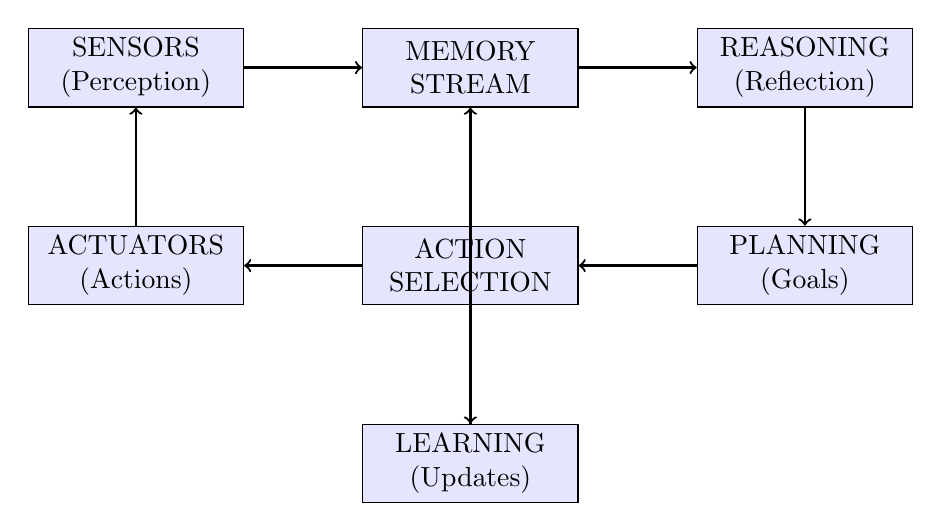
\begin{tikzpicture}[node distance=1.5cm, auto,
    block/.style={rectangle, draw, fill=blue!10, text width=2.5cm, text centered, minimum height=1cm},
    arrow/.style={->, thick}]
    
    \node[block] (sensors) {SENSORS\\(Perception)};
    \node[block, right=of sensors] (memory) {MEMORY\\STREAM};
    \node[block, right=of memory] (reasoning) {REASONING\\(Reflection)};
    \node[block, below=of reasoning] (planning) {PLANNING\\(Goals)};
    \node[block, left=of planning] (action) {ACTION\\SELECTION};
    \node[block, left=of action] (actuators) {ACTUATORS\\(Actions)};
    \node[block, below=of action] (learning) {LEARNING\\(Updates)};
    
    \draw[arrow] (sensors) -- (memory);
    \draw[arrow] (memory) -- (reasoning);
    \draw[arrow] (reasoning) -- (planning);
    \draw[arrow] (planning) -- (action);
    \draw[arrow] (action) -- (actuators);
    \draw[arrow] (actuators) -- (sensors);
    \draw[arrow] (action) -- (learning);
    \draw[arrow] (learning) -- (memory);
    
\end{tikzpicture}
\end{center}

\newpage
%----------------------------------------------------------
\section{Agent Characteristics}
%----------------------------------------------------------

\subsection{Internal Characteristics (Mental State)}

\begin{table}[h]
\centering
\begin{tabular}{|l|l|p{6cm}|}
\hline
\textbf{Characteristic} & \textbf{Type} & \textbf{Description} \\
\hline
Personality Traits & Static & Big Five: Openness, Conscientiousness, Extraversion, Agreeableness, Neuroticism \\
Current Emotion & Dynamic & Mood state updated by events \\
Goals & Dynamic & Short-term and long-term objectives \\
Memory Stream & Persistent & Time-stamped observations with importance scores \\
Relationships & Dynamic & Map of relationship strengths with other agents \\
Energy Level & Dynamic & Physical/mental fatigue (0-100) \\
\hline
\end{tabular}
\caption{Internal Agent Characteristics}
\end{table}

\subsection{External Characteristics (Observable)}

\begin{table}[h]
\centering
\begin{tabular}{|l|l|}
\hline
\textbf{Characteristic} & \textbf{Description} \\
\hline
Location & Current position in the base \\
Activity & Current action being performed \\
Expression & Visible emotional state \\
Interactions & Ongoing conversations or collaborations \\
\hline
\end{tabular}
\caption{External Agent Characteristics}
\end{table}

\subsection{The 8 Agents}

\begin{table}[h]
\centering
\small
\begin{tabular}{|l|l|l|p{4cm}|}
\hline
\textbf{Agent} & \textbf{Role} & \textbf{Key Traits} & \textbf{Internal Conflict} \\
\hline
Cdr. Vikram Sharma & Mission Commander & Disciplined, decisive & Hiding health condition \\
Dr. Ananya Iyer & Botanist/Life Support & Nurturing, optimistic & Guilt over leaving family \\
TARA & AI Assistant & Curious, evolving & Questioning consciousness \\
Aditya Reddy & Systems Engineer & Practical, homesick & Wants early return \\
Dr. Arjun Menon & Flight Surgeon & Calm, perceptive & Dual loyalty conflict \\
Kabir Saxena & Geologist/Mining & Rebellious, brilliant & Proving worth \\
Rohan Pillai & Communications & Cheerful, social & Carrying secret information \\
Priya Nair & Crew Welfare & Empathetic, trusted & Burden of secrets \\
\hline
\end{tabular}
\caption{Agent Profiles}
\end{table}

\newpage
%----------------------------------------------------------
\section{PARL Framework Implementation}
%----------------------------------------------------------

The agents operate using the PARL (Perception, Action, Reasoning, Learning) framework:

\subsection{Perception Module}
\begin{verbatim}
Input: Environment state
Output: Observations list

Process:
1. Scan current location for agents, objects, events
2. Check personal status (energy, mood, messages)
3. Note current time and scheduled activities
4. Create timestamped observation records
\end{verbatim}

\subsection{Action Module}
\begin{verbatim}
Input: Selected action from planning
Output: Environment modification

Available Actions:
- Movement: Navigate between locations
- Communication: Talk, listen, broadcast
- Work: Perform role-specific tasks
- Social: Build relationships, resolve conflicts
- Self-care: Rest, eat, recreation
\end{verbatim}

\subsection{Reasoning Module}
\begin{verbatim}
Input: Current observations + Retrieved memories
Output: Insights and plans

Process:
1. Retrieve relevant memories (recency, importance, relevance)
2. Generate reflections (high-level insights)
3. Evaluate current goals
4. Create/update action plans
\end{verbatim}

\subsection{Learning Module}
\begin{verbatim}
Input: Action outcomes
Output: Updated memory weights

Process:
1. Store new experiences in memory stream
2. Calculate importance scores for memories
3. Update relationship strengths based on interactions
4. Consolidate old memories (compression)
\end{verbatim}

\newpage
%----------------------------------------------------------
\section{Frontend and Backend Architecture}
%----------------------------------------------------------

\subsection{System Architecture}

\begin{center}
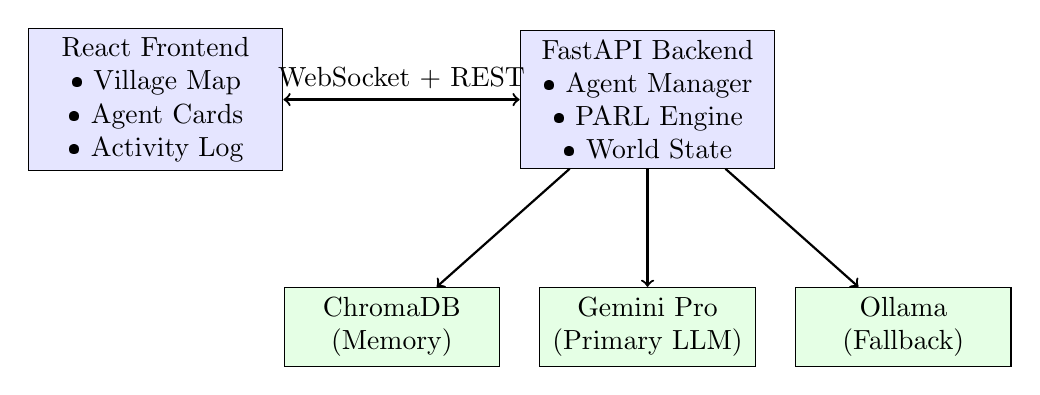
\begin{tikzpicture}[node distance=2cm, auto,
    box/.style={rectangle, draw, fill=blue!10, text width=3cm, text centered, minimum height=1.5cm},
    smallbox/.style={rectangle, draw, fill=green!10, text width=2.5cm, text centered, minimum height=1cm}]
    
    \node[box] (frontend) {React Frontend\\• Village Map\\• Agent Cards\\• Activity Log};
    \node[box, right=3cm of frontend] (backend) {FastAPI Backend\\• Agent Manager\\• PARL Engine\\• World State};
    
    \node[smallbox, below=1.5cm of backend] (gemini) {Gemini Pro\\(Primary LLM)};
    \node[smallbox, right=0.5cm of gemini] (ollama) {Ollama\\(Fallback)};
    \node[smallbox, left=0.5cm of gemini] (chromadb) {ChromaDB\\(Memory)};
    
    \draw[<->, thick] (frontend) -- node[above] {WebSocket + REST} (backend);
    \draw[->, thick] (backend) -- (gemini);
    \draw[->, thick] (backend) -- (ollama);
    \draw[->, thick] (backend) -- (chromadb);
    
\end{tikzpicture}
\end{center}

\subsection{Technology Stack}

\begin{table}[h]
\centering
\begin{tabular}{|l|l|}
\hline
\textbf{Layer} & \textbf{Technology} \\
\hline
Frontend & React + Vite \\
Backend & Python + FastAPI \\
Real-time & WebSocket \\
Primary LLM & Google Gemini Pro \\
Fallback LLM & Ollama (local) \\
Memory Store & ChromaDB (vector DB) \\
Tracing & LangChain + LangSmith \\
\hline
\end{tabular}
\caption{Technology Stack}
\end{table}

\subsection{Data Flow}

\begin{enumerate}
    \item \textbf{User Input} — Start simulation with parameters
    \item \textbf{Backend} — Initialize agents with personalities
    \item \textbf{Simulation Loop}:
    \begin{itemize}
        \item Each agent: Perceive → Reason → Act → Learn
        \item Update world state
        \item Emit events via WebSocket
    \end{itemize}
    \item \textbf{Frontend} — Render agent positions, activities, conversations
    \item \textbf{Logging} — Store interactions for analysis
\end{enumerate}

%----------------------------------------------------------
\section*{References}
%----------------------------------------------------------

\begin{enumerate}
    \item Park, J.S., et al. (2023). ``Generative Agents: Interactive Simulacra of Human Behavior.'' \textit{arXiv:2304.03442}
    \item Russell, S., \& Norvig, P. (2020). ``Artificial Intelligence: A Modern Approach.'' 4th Edition
    \item ISRO. (2023). ``Chandrayaan-3 Mission Overview.'' Indian Space Research Organisation
\end{enumerate}

\vfill
\begin{center}
\textit{Document Version: 1.0 | Last Updated: January 2026}
\end{center}

\end{document}
